\documentclass[a4paper,10pt]{report}
\usepackage[english]{babel}
\usepackage[utf8]{inputenc}
\usepackage{listings}
\usepackage{enumitem}
\usepackage{graphicx}
\usepackage{amsmath}

\graphicspath{{./figures}}


\title{A-FMM User Guide}
\author{Marco Passoni}
\date{}

\begin{document}

\maketitle

\tableofcontents

\chapter{Algorithm} 

Aperiodic-Fourier Modal Method is a frequency domain method based on the Scattering Matrix approach. 

This method can be used to solve Maxwell equations on any structure, provided it can be represented as a multilayer. Inside each layer, the dielectric constant along the stacking direction (let's call it $z$) has to be uniform. Variation of the dielectric constant in the plane perpendicular to the stacking direction (the $xy$) plane is instead permitted.

\begin{figure}
\centering
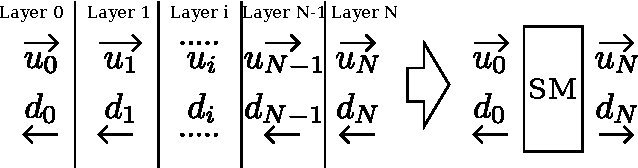
\includegraphics[width=0.8\textwidth]{figures/SM.pdf}
\caption{scattering matrix}
\label{fig:SM}
\end{figure} 

The basic working principle is as follows. Firstly, the fields in each layer (for now assumed infinite in the $z$ direction) are expressed as a sum of forward and backward propagating plane waves (expansion on a Fourier basis). Secondly, the boundary conditions are applied to each interface, linking together the fields in each layer. The output of the code is the scattering matrix $S$, a matrix that connects the Fourier expansion of the fields outgoing from the structure to the one of the incoming fields:
\begin{equation} \label{eq:SM_def}
\left[ \begin{array}{c} u_N \\ d_0 \end{array} \right] =
S \left[ \begin{array}{c} u_0 \\ d_N \end{array} \right] = \left[ \begin{array}{cc} S_{11} & S_{12} \\ S_{21} & S_{22} \end{array} \right] \left[ \begin{array}{c} u_0 \\ d_N \end{array} \right]
\end{equation}  
where $u_i$ and $d_i$ are the coefficient of the Fourier expansion in the $i^{th}$ layer for the forward and backward propagating waves. 

If a total of $M$ elements of the Fourier expansion are retained, each $u_i$ and $d_i$ is a $2M$ vector (the factor $2$ account for the two different polarization states) and the Scattering Matrix $S$ is a $4M \times 4M$ matrix. 

Once the scattering matrix of a system is known, information such as reflection, transmission and diffraction in the open orders can be extracted. Since the scattering matrix gives the coupling coefficient between the input and output Fourier modes, getting such information is just a matter of taking the correct element in the scattering matrix and normalizing it with the ratio of the Poynting vectors between the selected modes. 

The A-FMM has its roots in the classical modal method for crossed gratings, firstly devised by L. Li \footnote{Li, Lifeng. "New formulation of the Fourier modal method for crossed surface-relief gratings." JOSA A 14.10 (1997): 2758-2767.} in 1997. The method was then updated by J.P. Hugonin and P. Lalanne \footnote{Hugonin, J. P., et al. "Fourier modal methods for modeling optical dielectric waveguides." Optical and Quantum Electronics 37.1-3 (2005): 107-119.} with the inclusion of a coordinate transformation. The role of the coordinate transformation is to map the entire $\mathbf{R}$ space ($\mathbf{R}^2$ for 3D calculation) to the finite computational cell. In this way the computational cell can contain an arbitrary dielectric constant distribution, which can still be treated with Fourier Methods but without crosstalk between adjacent cells.

The procedure involved in the A-FMM can be summarized as:
\begin{enumerate}
\itemsep0em 
\item Dividing the system in $N$ layers.
\item Solving the Maxwell equations in each layer, assuming homogeneity in the staking ($z$) direction, expanding the filed on a Fourier Basis. 
\item Using the solution found in 2, calculating the propagation matrix in each layer and the scattering matrix of each interface.
\item Using the recursion algorithm for the scattering matrix, calculating the scattering matrix of the full structure. 
\item Obtaining the desired quantities by post-processing of the scattering matrix. 
\end{enumerate}

A brief summary of every step will now be reported. Firstly, it is necessary to expand the fields in each layer as a sum over pseudo-Fourier basis \index{Fourier expansion}:
\begin{equation} \label{eq:Fourier_ex}
\Phi(x,y,z)= \sum_{n,m}=\Phi_{n,m}(z)\exp \left\{ i(k_x+\frac{2\pi n}{L_x})x+i(k_y+\frac{2\pi m}{L_y})y \right\}
\end{equation}
where $\Phi$ is a generic component of the electromagnetic fields, $k_x,k_y$ are the components of the wavector along the $x,y$ direction. The values $L_x$ and $L_y$ are the dimension of the computational cell. Due to the coordinate transformation they lack a physical meaning, but their values are still important in the definition of the basis for the pseudo-Fourier expansion, and remain as computational parameters.

Once the expansion is established, it can be inserted in the Maxwell equations to get the solution inside the single layer. After this substitution and a little manipulation it is possible to write:

\begin{subequations} \label{eq:def_sys}
\begin{equation} \label{eq:def_F}
-\frac{i}{k_0} \frac{\partial}{\partial z} 
\left[ \begin{array}{c}
E_x \\ E_y \\
\end{array} \right] = 
\left[ \begin{array}{cc}
\bar{K_x} \varepsilon^{-1} \bar{K_y}    & 1- \bar{K_x} \varepsilon^{-1} \bar{K_x} \\
\bar{K_y} \varepsilon^{-1} \bar{K_y} -1 &   -\bar{K_y} \varepsilon^{-1} \bar{K_x} \\
\end{array} \right]
\left[ \begin{array}{c}
 H_x \\ H_y \\
\end{array} \right] 
= F \left[ \begin{array}{c}
 H_x \\ H_y \\
\end{array} \right] 
 \end{equation}
\begin{equation} \label{eq:def_G}
-\frac{i}{k_0} \frac{\partial}{\partial z} 
\left[ \begin{array}{c}
H_x \\ H_y \\
\end{array} \right] = 
\left[ \begin{array}{cc}
 -\bar{K_x} \bar{K_y} & \bar{K_x}^2 - \varepsilon_{y,x} \\
 \varepsilon_{x,y} - \bar{K_y}^2 & \bar{K_x} \bar{K_y} \\
\end{array} \right]
\left[ \begin{array}{c}
E_x \\ E_y
\end{array} \right]
= G \left[ \begin{array}{c}
E_x \\ E_y
\end{array} \right]
\end{equation}
\end{subequations}
where $E_x,E_y,H_x,H_y$ are the vectors containing the Fourier expansion coefficients of the respective field, and $k_0= \omega/c$ is the vacuum wavevector of the radiation. The matrices $\varepsilon, \varepsilon_{x,y}$ and $\varepsilon_{y,x}$ are built with the Fourier transform of the dielectric function in the computational cell --- see ref.~\cite{li1997new} and App.~\ref{ap:coordinate_trans} for further details. The matrix $\bar{K_x}$ is built as:
\begin{equation} \label{eq:K_bar}
\bar{K_x} = F_x K_x,
\end{equation}
where $K_x$ is simply the matrix containing the wavevectors of the Fourier expansion ($K_x(g,g') = (k_x+g_x)\delta_{gg'}$) and $F_x$ is built from the Fourier coefficient of the derivative of the function used for the coordinate transformation --- see App~\ref{ap:coordinate_trans} for details. The matrix $F_y$ is built in an analogous way.

A further summary of Eq.~\ref{eq:def_F} and \ref{eq:def_G} is desirable. Focusing on solutions of $\Psi$ which have a $z$ dependence in the form $e^{i\gamma z}$ it is possible to write:
\begin{equation} \label{eq:eigenproblem}
FG \left[ \begin{array}{c} E_x \\ E_y \\ \end{array} \right] = \frac{\gamma^2}{k_0^2} \left[ \begin{array}{c} E_x \\ E_y \\ \end{array} \right],
\end{equation}
which takes the form of an eigenvalue problem concerning only the electric field components. The eigenvalues $\gamma^2/k_0^2$ are related to the propagation constant along $z$ of the eigenmodes of the layer, while the eigenvectors give the electric field profile of th modes. Since for every eigenvalue two solutions for $\gamma$ are possible --- forward and backward propagating --- only the solution satisfying $Re(\gamma)+Im(\gamma) > 0 $ will be considered and labeled with subscript $q$. \index{Eigenvalue problem}

Defining the vector $E=[E_x E_y]^T$ and the matrix $\tilde{E}$ containing as columns the eigenvectors of Eq. \ref{eq:eigenproblem}, the corresponding matrix $\tilde{H}$ for the magnetic filed can be expressed as:
\begin{equation} \label{eq:Htilde}
\tilde{H} = \frac{k_0}{\gamma} \tilde{E} 
\end{equation}
which contains the Fourier coefficient regarding the magnetic filed of the eigenmodes. 

At this point it is possible, after the definition of the vectors $u$ and $d$, containing, respectively, the amplitude of the forward and backward propagating modes inside the layer, to write the Fourier coefficients of the field at an arbitrary value $z$ as a function of $u$ and $d$:
\begin{equation}
\left[ \begin{array}{c} E \\ H \\ \end{array} \right]_z = 
\left[ \begin{array}{cc} \tilde{E} & \tilde{E} \\ \tilde{H} & -\tilde{H} \\  \end{array} \right] 
\left[ \begin{array}{c} u \\ d \\ \end{array} \right]_z
\end{equation}  

Currently a method of connecting the vectors $u$ and $d$ at different $z$ values (both in the same layer or in different ones) is still lacking. In the following the scattering matrix for both cases will be built. 

The easiest case is when the two values of $z$ are in the same layer. In this condition, the values of $u$ and $d$ at $z$ and $z'$ are simply linked with a propagation scattering matrix:
\begin{equation} \label{eq:prop_matrix}
\left[ \begin{array}{c} u' \\ d \end{array} \right] =
\left[ \begin{array}{cc} \exp[i\Gamma(z-z') & 0 \\ 0 & \exp[i\Gamma(z-z')] \\ \end{array} \right]
\left[ \begin{array}{c} u \\ d' \end{array} \right]
\end{equation}
where $\Gamma$ is simply the matrix with the propagation constants of the modes $\gamma$ on the diagonal. 

When the two $z$ values lie in different layers the calculations are a bit more complex. However, is it possible to demonstrate that the scattering matrix of a single interface between two layers can be written as (normal variables refer to the first layer, the primed to the second):
\begin{equation} \label{eq:interface_matrix}
\left[ \begin{array}{cc} S_{11} & S_{12} \\ S_{21} & S_{22} \\ \end{array} \right] =
\left[ \begin{array}{cc} T_+ - T_-T_+^{-1}T_- & T_- T_+^{-1} \\ -T_+^{-1}T_- & T_+^{-1} \\ \end{array} \right],
\end{equation}
where $T_\pm$ is defined as:
\begin{equation}
T_\pm=\frac{1}{2} \left( \tilde{E'}^{-1}\tilde{E} \pm \tilde{H'}^{-1}\tilde{H}  \right).
\end{equation}

Now that both propagation and interface scattering matrices are defined, in order to connect the $u$ and $d$ vectors at different $z$ values all that is needed is a recursion algorithm to join together two matrices, allowing the scattering matrix of the complete system to be built up  piece by piece. In details, the recursion algorithm joining to scattering matrices $S$ and $s$ in the total scattering matrix $S^T$ is:
\begin{subequations}
\begin{equation}
S^T_{11} = s_{11}(1-S_{12} s_{21})^{-1} S_{11}
\end{equation}
\begin{equation}
S^T_{12} = s_{12} +s_{11} (1-S_{12} s_{21})^{-1} S_{12} s_{22}
\end{equation}
\begin{equation}
S^T_{21} = S_{21} +  S_{22}(1-s_{21} S_{12})^{-1} s_{21} S_{11}
\end{equation}
\begin{equation}
S^T_{22} = S_{22}(1-s_{21} S_{12})^{-1} s_{22}
\end{equation}
\end{subequations}
It is worth noting that this relation, together with the fact that no diverging exponential appears in the propagation matrix \ref{eq:prop_matrix}, ensures the numerical stability of the S-matrix, at variance with other schemes (i.e. T-matrix).

Once the scattering matrix of the entire system is known, informations such a coupling strength between one input mode  and one output mode are easily calculated. As an example, the fraction of power scattered from a mode $m$ to a mode $n$ can be calculated as:
\begin{equation} \label{eq:cacl_stattering}
\frac{P_n}{P_m}=|S(n,m)|^2 \frac{\mathcal{P}_n}{\mathcal{P}_m}
\end{equation}
where $S(n,m)$ is the relevant S-matrix element and the quantities $\mathcal{P}_i$ are the $z$-component of the Poyting vector referring to the $i$ mode. This component can be calculated as:
%\begin{equation} \label{eq:poynting_mode}
%\mathcal{P}_i=\sum_n E_x(n)H_x^*(n)+E_y(n)H_x^*(n)
%\end{equation}
\begin{equation} \label{eq:poynting_mode}
\mathcal{P}= \frac{1}{2} Re \left[ E_x^TH_y^*-E_y^TH_x^* \right]
\end{equation}
where $E_x,E_y,H_x$ and $H_y$ are the vectors of the Fourier components of the mode under consideration. 

Speaking of the Poynting vector, it is also possible to calculate the total Poynting vector as a function of $z$. This is a little more complex than before (where only the Poyting vector relative to a single mode was calculated) since now every mode (forward and backward propagating), together with their interference, has to be considered. In the end, the total Poyting vector $\mathcal{P}^{TOT}_z$ can be expressed as:
\begin{equation} \label{Poynting_tot}
\mathcal{P}^{TOT}_z= \frac{1}{2} Re \left\{
\left[ \begin{array}{cc} u & d \\  \end{array} \right]_z
\left[ \begin{array}{cc} \tilde{\mathcal{P}} & -\tilde{\mathcal{P}} \\ \tilde{\mathcal{P}} & -\tilde{\mathcal{P}} \\  \end{array} \right]
\left[ \begin{array}{c} u^* \\ d^* \\  \end{array} \right]_z \right\}
\end{equation}
where $\tilde{\mathcal{P}}$ is a matrix whose elements are defined as:
\begin{equation} \label{eq:P_matrix}
\tilde{\mathcal{P}}_{nn'} = \sum_k \left[ \tilde{E}_x(k,n)\tilde{H}_y^*(k,n') - \tilde{E}_y(k,n)\tilde{H}_x^*(k,n') \right]
\end{equation}

However, the practical use of Eq.~\ref{Poynting_tot} to get the total Poyting vector requires the calculation of $u_z$ and $d_z$, namely the vectors containing the coefficients of the forward and backward propagating modes at $z$. In order to do that, two S-matrices have to be built. The first $S$ is the matrix linking the beginning of the structure to the desired $z$ coordinate, while the second $S'$ links this $z$ coordinate to the end of the structure. Once those S-matrices are known, the vectors $u_z$ and $d_z$ can be calculated from the input vector $u$ and $d'$ as:
\begin{subequations}
\begin{equation}
u_z=\left(1-S_{12}S'_{21} \right)^{-1} \left(S_{11}u + S_{12}d' \right)
\end{equation}
\begin{equation}
d_z=\left(1-S'_{21}S_{12} \right)^{-1} \left(S'_{21}u + S'_{22}d' \right)
\end{equation}
\end{subequations}


One last, but very important, application of the scattering matrix is the calculation of the photonic bands in periodic structures. This can be done by solving a generalized eigenvalue problem derived from the S-matrix of the unit cell. The eigenvalue problem is obtained imposed Bloch boundary conditions on the fields on the two side of the structure:
\begin{equation} \label{eq:Bloch_cond}
\left[ \begin{array}{cc} u' \\ d' \\ \end{array} \right] = 
e^{ik\Lambda} \left[ \begin{array}{cc} u \\ d \\ \end{array} \right]
\end{equation}
where $k$ and $\Lambda$ are the Bloch vector and the period along the $z$ direction, respectively. 
Inserting the Bloch boundary condition in the definition of the scattering matrix (Eq.~\ref{eq:SM_def}) easily yields:
\begin{equation} \label{eq:SM_Bloch_eig}
\left[ \begin{array}{cc} S_{11} & 0 \\ S_{21} & -1 \\ \end{array} \right]
\left[ \begin{array}{c} u \\ d \\ \end{array} \right] = e^{ik\Lambda}
\left[ \begin{array}{cc} 1 & -S_{12} \\ 0 & -S_{22} \\ \end{array} \right]
\left[ \begin{array}{c} u \\ d \\ \end{array} \right] 
\end{equation}
which can be solved to obtain the Bloch vector $k$ for given frequency. 

The Aperiodic Fourier Modal Method is the main instrument for the research on slow light in silicon grating waveguides, both for calculation of photonic bands and transmission through finite size structures.

\chapter{The software}

\section{examples}

\subsection{Mode of a slab waveguide} \label{ex:slab_modes}
\textbf{File:} \texttt{slab\_modes.py} \\
This example is designed to illustrate the basic usage of the \texttt{creator} and \texttt{layer} classes. This script calculates the effective indexes as a function of energy of a planar slab waveguide. The script works as follows:
\begin{enumerate}
\itemsep0em 
\item Some parameters (truncation order, energy vector) are defined;
\item A creator instance \texttt{cr} is initialized;
\item The structure is defined calling the slab method of \texttt{cr} --- a number of methods for the creator class are built in the code;
\item A layer instance in created;
\item The transformation of coordinate is applied;
\item Loop over energies is started, inside the loop:
\begin{enumerate}
\itemsep0em 
\item The \texttt{mode} method of the \texttt{layer} class is used to calculate the modes;
\item Effective indexes are retrieved from the \texttt{gamma} vector of the \texttt{layer} instance and sorted;
\item Results are printed;
\end{enumerate}
\end{enumerate}

\subsection{Mode of a ridge waveguide}
\textbf{File:} \texttt{ridge\_modes.py} \\
This example has the same structure as the previous one, but the analyzed structure is a ridge waveguide, thus requiring a 2D cell. 

\subsection{Reflection and transmission of a 1D grating. Wavelenght and angle} \label{ex:grating1d}
\textbf{File:} \texttt{1D\_grating.py} \\
This example is designed to illustrate the basic usage of the stack class and how to calculate coupling between different input and output modes (such as reflection and transmission). The scripts is organized as follows: 
\begin{enumerate}
\itemsep0em 
\item Definition of the relevant parameters (truncation order, vectors for energies and angle sweeps);
\item Definition of the layers used in the structure;
\item Creation of and instance if the \texttt{stack} class, defining the full structure and containing all the methods for solving it:
\begin{enumerate}
\itemsep0em
\item A list of layers composing the structure is contructed;
\item A list of the thicknesses of each layer is constructed (length the same as list of layer). The thickness values of the first and last layers are useful only for plotting purposes, and have no effect whatsoever on the calculation; 
\item A stack object is created using the these two lists as inputs;
\item The method \texttt{count\_interface} of the \texttt{stack} object is called. This is a necessary step right after a stack definition;
\item The method \texttt{plot\_stack} is called to plot the reconstructed epsilon of the structure, output in a pdf file;
\end{enumerate}
\item The loops over energies and angle are started:
\begin{enumerate}
\itemsep0em
\item The scattering matrix is constructed calling the \texttt{solve} method of the \texttt{stack} class. Inputs in this case are energy (mandatory) and parallel  wavevector (optional, assumed 0 if missing).
\item Reflection and transmission between relevant modes are then extracted using the appropriate methods (\texttt{get\_T} and \texttt{get\_R}).
\item Results are printed to screen. 
\end{enumerate}
\end{enumerate}
Some notes on this script have to be made. First, note than to set the angle of incidence it is necessary to specify the parallel $x$($y$) wavevector. This wavevector is expressed in unit of $1/L_x$($1/L_y$) and the index of refraction has to be inserted manually.
Second, an observation on the reading of the results with \texttt{get\_R}. When the first an last layer are not patterned, the eigenstates of those layer are simple plane waves (in number 2*NPW, due to polarization). The first NPW modes are polarized (E field) along $x$, the second NPW along $y$. Inside each bloch, the modes are ordered following the dictionary G (which can be printed de-commenting the commented lines in the example). The 0,0 order is at the center of each block, thus at NPW/2 and 3/2*NPW (which one is TE and TM depends on which wavector is inserted in the calculation). Furthermore, it is important to use the option \texttt{ordered='no'}, otherwise the modes are ordered in decreasing effective index, resulting in a lack of consistence when a sweep in angle is made.  

\subsection{Reflection and transmission of a 1D grating. Wavelenght and angle}
\textbf{File:} \texttt{2D\_grating.py} \\
This is the 2D version of the previous example. It requires much more computational effort, but is otherwise totally identical.

\subsection{PML implementation test: reflection and transmission in waveguide}
\textbf{File:} \texttt{pml\_test.py} \\
This script illustrate the use of the complex coordinate transformation which acts as a PML around the simulation regions, allowing the treatment of structure in which the scattering losses are consistent. It is also the prototype of the calculation of transmission and reflection from a waveguide structure. The script is built following the benchmark of Hugonin \textit{et al.}\footnote{Hugonin, Jean Paul, and Philippe Lalanne. "Perfectly matched layers as nonlinear coordinate transforms: a generalized formalization." JOSA A 22.9 (2005): 1844-1849.} The script is  The script is structures as follows:
\begin{enumerate}
\itemsep0em
\item A series of layer instances are defined (see Ex.\ref{ex:slab_modes}), one for each different segment of the structure. 
\item A stack instance is created, using as input a list of layers and one of thicknesses. 
\item The complex coordinate transformation is applied in the $x$ direction. 
\item The scattering matrix is calculated (\texttt{solve})
\item Reflection and transmission are obtained (see Ex.~\ref{ex:grating1d}).
\item Fields inside the structure are plotted. 
\end{enumerate}
A few observations have to be made. This this time the function \texttt{get\_R} (and \texttt{get\_T}) are called with the option \texttt{ordered='yes'} (whcih is also the default option). IN this way the modes in the reference layer are ordered in decreasing effective index. Thus the 1 mode is the fundamental one one (fundamental TE in this specific case), 2 second one (fundamental TM in this case) and so on. The same syntax is used in the \texttt{plot\_E} command.

 




\chapter{Reference Guide}
In this chapter a detailed explanation of the module is provided. For each sub-module a summary of the classes and function involved can be found, together with details on the most common functions.
\section{Module composition}
The A-FMM module in turn composed by different submodules:
\begin{itemize}
\item creator module: Contain the creator class, used to define the dielectric costant of the single layer.   
\item layer module: Contain the layer class, used to solve the Maxwell equation inside each single layer. It requires a creator instance to be initialized.
\item scattering module: Contain the S\_matrix class. All method for scattering matrix creation and manipulation are here implemented.  
\item satck module: Contain the stack class, used to calculate the Scattering Matrix and related quantities of the hole structure. It is initialize from a collection of layer instances.
\item sub\_sm module: Contains auxiliary function that are called in more than one module. It is non loaded by default when loading A\_FMM.
\end{itemize}

\section{S\_matrix class}
\subsection{Initialization}
This class contains the definition of the scattering matrix object and all method for scattering matrix manipulation. The scattering matrix is an object relating the amplitudes of the incoming end outgoing modes of a structure. It presets itself as following:
\begin{equation} \label{eq:S_matrix_def}
\left[
\begin{array}{c}
u' \\
d  \\
\end{array} 
 \right] = \left[
 \begin{array}{cc}
S_{11} & S_{12} \\
S_{21} & S_{22} \\
\end{array}
 \right]
 \left[
\begin{array}{c}
u \\
d' \\
\end{array} 
\right]
\end{equation}
following the convention of figure \ref{fig:SM_conv}.
\begin{figure}
\centering
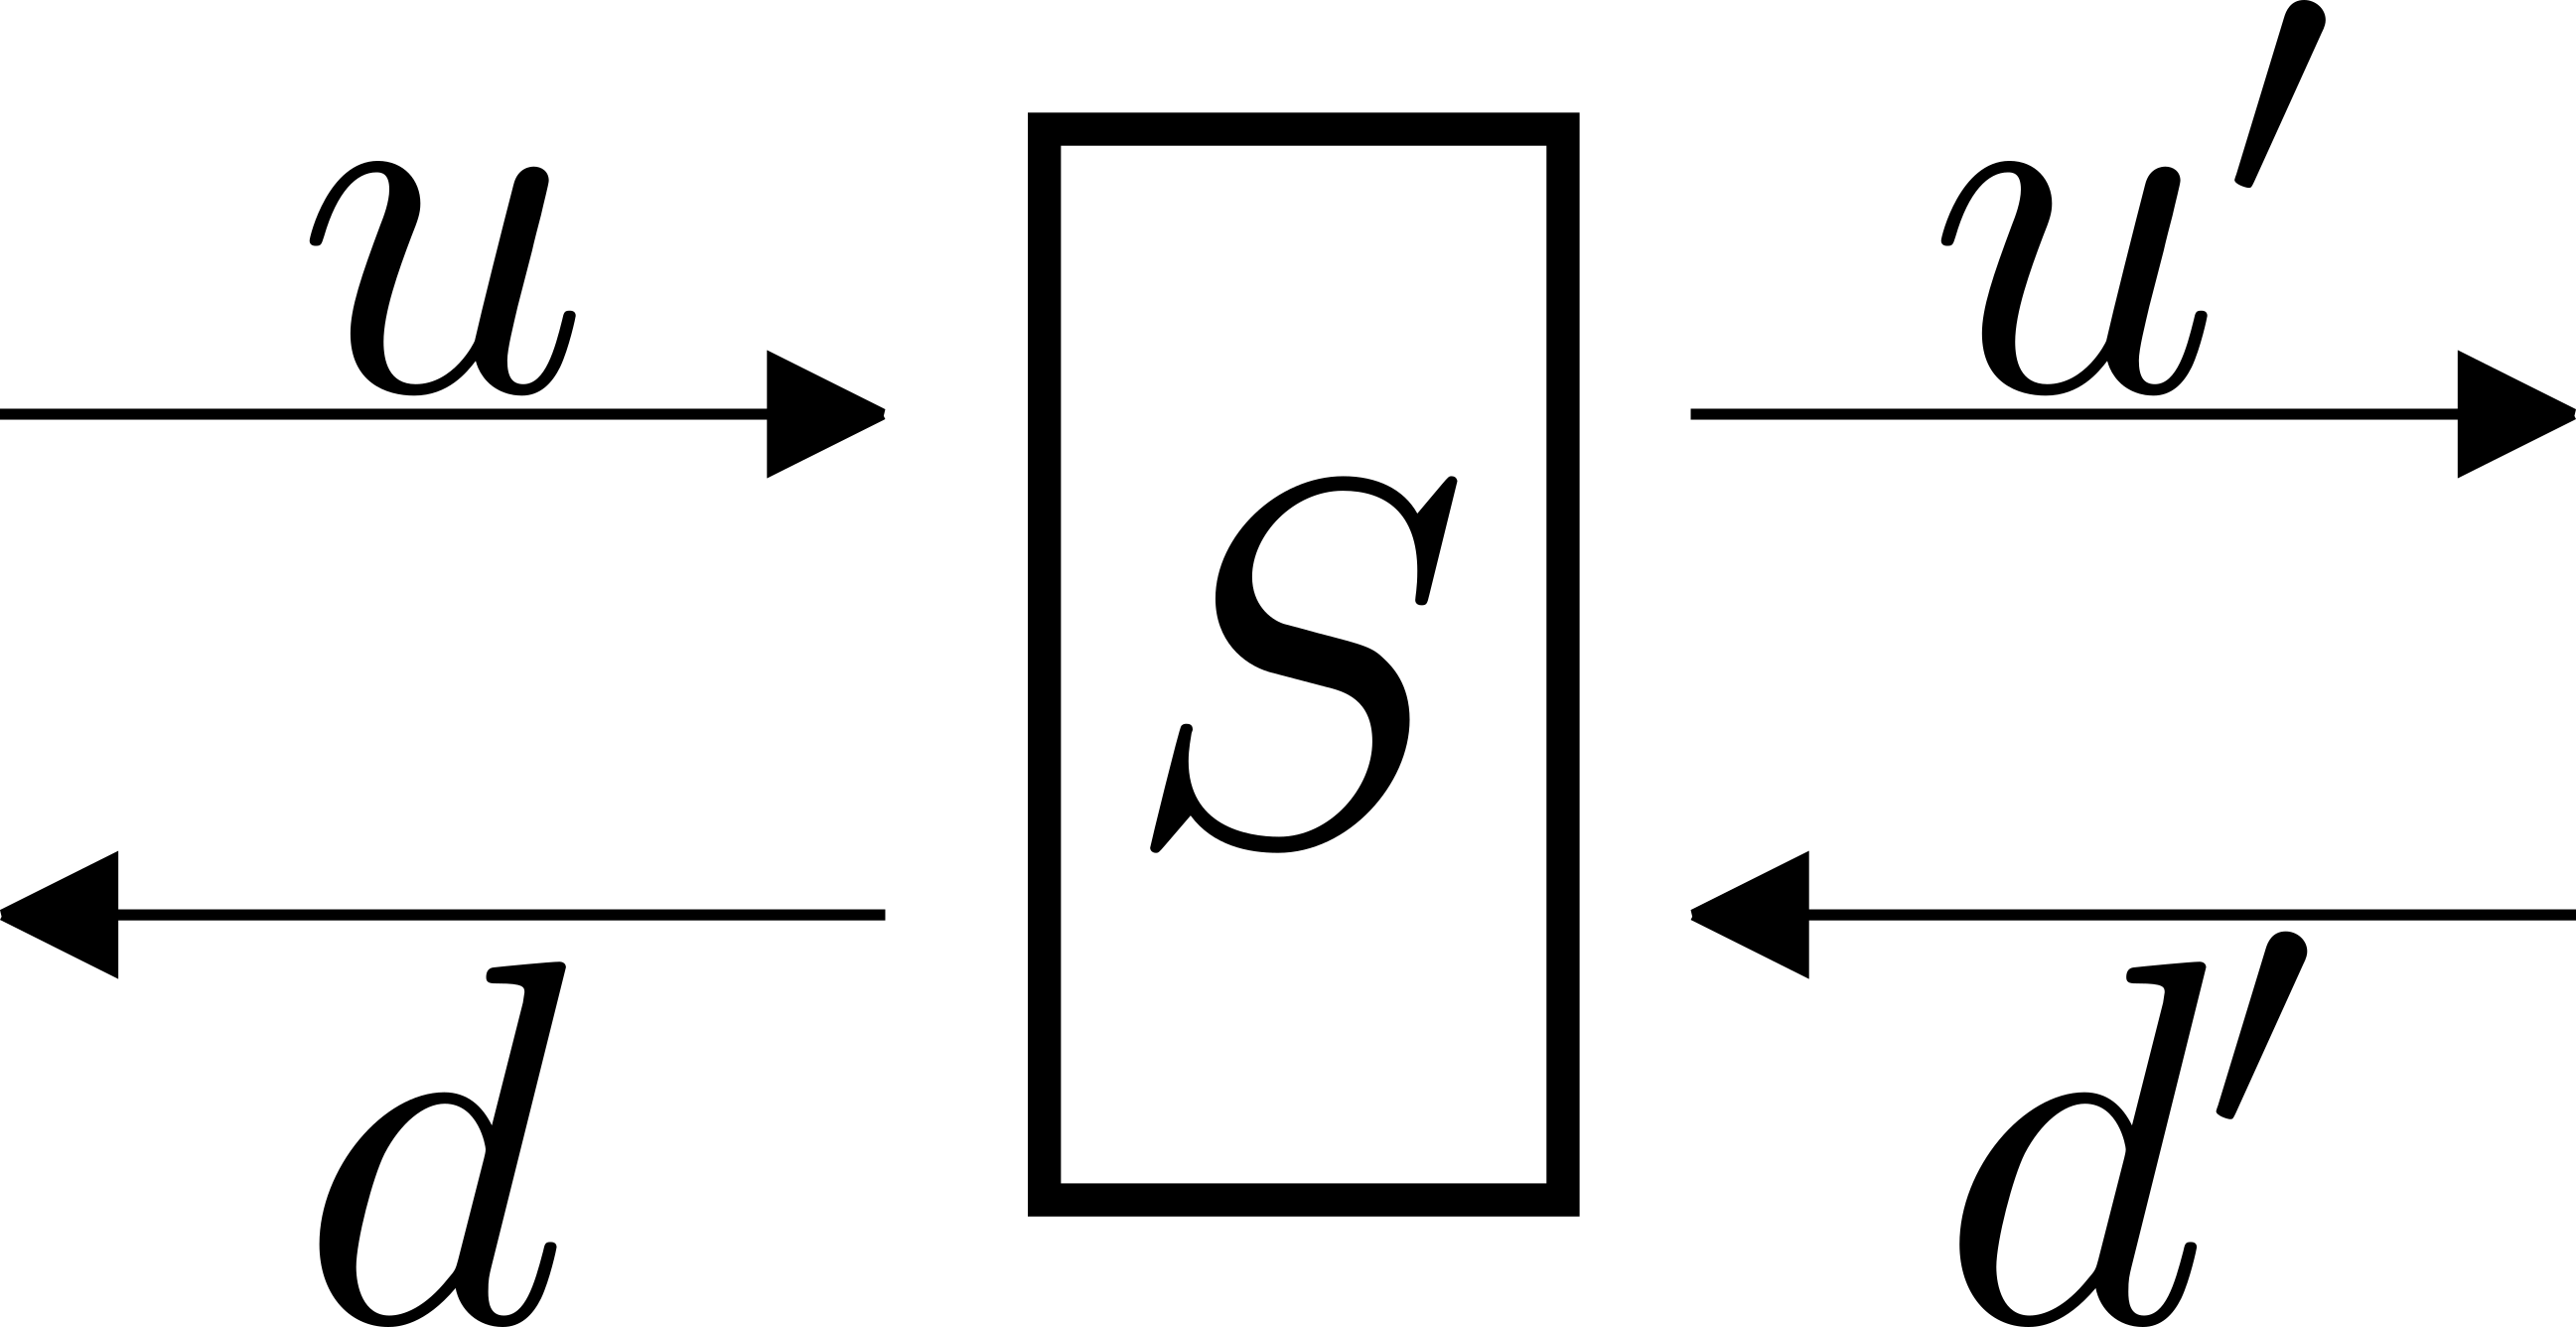
\includegraphics[width=0.5\textwidth]{figures/S.png}
\caption{Convention adopted for the scattering matrix formalism.} \label{fig:SM_conv}
\end{figure}
An instance is initialized as:
\begin{lstlisting}[language=Python]
S=S_matrix(N)
\end{lstlisting}
where \texttt{N} is the dimension of the four $N \times N$ matrices composing the scattering matrix. Each of this matrix is saved as an \texttt{numpy.ndarray} as an attribute of the S\_matrix object. For example to the $(1,2)$ element of the $S_{21}$ matrix is accessed as \texttt{S.S21[1,2]}.

\subsection{Method}
\begin{lstlisting}[language=Python,basicstyle=\ttfamily\Large]
add(s)
\end{lstlisting}
Takes as input an other instance of the S\_matrix class s, which is then joined to the right to the scattering matrix that calls the method.

\begin{lstlisting}[language=Python,basicstyle=\ttfamily\Large]
add_left(s)
\end{lstlisting}
Same as \texttt{add} but s matrix is joined to the left.

\begin{lstlisting}[language=Python,basicstyle=\ttfamily\Large]
add_uniform(lay,d)
\end{lstlisting}
Takes as input:
\begin{itemize}[noitemsep,topsep=0pt,parsep=0pt,partopsep=0pt]
\item \texttt{lay}: An instance of the layer class;
\item \texttt{d}: A float representing the thickness of the layer.
\end{itemize}
This method creates the scattering matrix for propagation trough a layer \texttt{lay} of thickness \texttt{d}, and then joins it to the right of the scattering matrix that calls the method.

\begin{lstlisting}[language=Python,basicstyle=\ttfamily\Large]
add_uniform_left(lay,d)
\end{lstlisting}
Same as \texttt{add\_uniform} but joins to the left.





\section{Layer Class}
\subsection{Initialization}
This layer class is contained in the layer module. It is responsible for definition of the single layer inside the scattering matrix approach. It also contains the methods for adding the coordinate transform an plotting of the mode fields. The different layer are:
\begin{lstlisting}[language=Python]
lay=layer(Nx,Ny,creator,Nyx=1.0)
\end{lstlisting}
which is the standard implementation of the class. A \texttt{creator} object is needed for the creation, and all the calculation for the Fourier transform are done analytically. The parameter for the initialization are:
\begin{itemize}[noitemsep,topsep=0pt,parsep=0pt,partopsep=0pt]
\item \texttt{Nx,Ny}: Trucation order respectively in $x$ and $y$ direction. Actual number of plane waves is $(2N_x+1)(2N_y+1)$.
\item \texttt{creator}: The creator instance describing the dielectric function.
\item \texttt{Nyx}: Ratio between the cell period in $y$ and $x$ direction (default is 1.0).
\end{itemize}

\begin{lstlisting}[language=Python]
lay=layer_num(Nx,Ny,func,args=(),Nyx=1.0,NX=1024,NY=1024)
\end{lstlisting}
Implementation in which the Fourier transforms for the layer are handled numerically. It is more versatile than the standard implementation, albeit should be less precise. The profile of the dielectric is obtained from the function \texttt{func}. The objects needed are:
\begin{itemize}[noitemsep,topsep=0pt,parsep=0pt,partopsep=0pt]
\item \texttt{Nx,Ny}: Integers, trucation order respectively in $x$ and $y$ direction. Actual number of plane waves is $(2N_x+1)(2N_y+1)$.
\item \texttt{func}: Function which defines the dielectric constant. It has to be in the form \texttt{func=func(x,y,..)}. After x and y additional parameters can be defined in the function and passed in \texttt{args}. Domain of the function in -0.5:0.5 in x and -0.5*Nyx:0.5*Nyx in y. 
\item \texttt{Nyx}: Ratio between the cell period in $y$ and $x$ direction (default is 1.0).
\item \texttt{args}: Tuple containing eventual additional parameters for \texttt{func}.
\item \texttt{NX,NY}: Integers, number of point in each direction used for numerical integration in the Fourier transforms.
\end{itemize}

\begin{lstlisting}[language=Python]
lay=layer_uniform(Nx,Ny,eps,Nyx=1.0)
\end{lstlisting}
Implementation of the uniform layer. It is implemented on is own because in this way its definition and solution are much faster. The parameters are:
\begin{itemize}[noitemsep,topsep=0pt,parsep=0pt,partopsep=0pt]
\item \texttt{Nx,Ny}: Trucation order respectively in $x$ and $y$ direction. Actual number of plane waves is $(2N_x+1)(2N_y+1)$.
\item \texttt{eps}: The dielectric constant of the uniform layer. Can be complex. 
\item \texttt{Nyx}: Ratio between the cell period in $y$ and $x$ direction (default is 1.0).
\end{itemize}
 


When initializing the layer class all the matrices involve in the eigenvalue problem for the layer are created.
\subsection{Fundamental Methods}
\begin{lstlisting}[language=Python,basicstyle=\ttfamily\Large]
trasform(ex=0,ey=0)
\end{lstlisting}
Add the real coordinate transform.
\begin{itemize}[noitemsep,topsep=0pt,parsep=0pt,partopsep=0pt]
\item \texttt{ex,ey}: Respectively the width of the untransformed region in $x$ and $y$ direction. If not specified transformation in not applied in that direction.
\end{itemize}

\begin{lstlisting}[language=Python,basicstyle=\ttfamily\Large]
trasform_complex(ex=0,ey=0)
\end{lstlisting}
Add the complex coordinate transform simulating PML boundary conditions. 
\begin{itemize}[noitemsep,topsep=0pt,parsep=0pt,partopsep=0pt]
\item \texttt{ex,ey}: Respectively the width of the untransformed region in $x$ and $y$ direction. If not specified transformation in not applied in that direction.
\end{itemize}

\begin{lstlisting}[language=Python,basicstyle=\ttfamily\Large]
mode(k0,kx=0.0,ky=0.0,v=1)
\end{lstlisting}
Solve the eigenvalue problem of the layer.
\begin{itemize}[noitemsep,topsep=0pt,parsep=0pt,partopsep=0pt]
\item \texttt{k0}: Energy of the mode
\item \texttt{kx,ky}: Respectively the lateral wavevector in the $x$ and $y$ direction (in unit of inverse of the period).
\item  \texttt{v}: If equal to 0 only eigenvalue are calculated. Useful when interested only in propagation constant of the mode of the single layer. Default is 1.
\end{itemize}
create three new attributes of the class layer:
\begin{itemize}[noitemsep,topsep=0pt,parsep=0pt,partopsep=0pt]
\item \texttt{W}: Vector of the eigenvalues (effective indexes of modes squared). 
\item \texttt{V}: Matrix of electric eigenvectors of the modes. \texttt{V[:,i]} is the vector to the $i^{th}$ mode.
\item \texttt{VH}: Matrix of magnetic eigenvectors of the modes. Same convention as \texttt{V}.
\end{itemize}

\begin{lstlisting}[language=Python,basicstyle=\ttfamily\Large]
eps_plot(pdf=None,N=200,s=1.0)
\end{lstlisting}
Plot dielectric function profile reconstructed from fourier transform.
\begin{itemize}[noitemsep,topsep=0pt,parsep=0pt,partopsep=0pt]
\item \texttt{pdf}: Name of the pdf file used to save the figure (string, without the .pdf).
\item \texttt{N}: Width in pixel of the cell. Default 200.
\item \texttt{s}: Number of fundamental cells plotted. Default 1.
\end{itemize}

\begin{lstlisting}[language=Python,basicstyle=\ttfamily\Large]
plot_E(pdf,i,N=100,s=1,func=np.abs)
\end{lstlisting}
Plot electric field profile of selected mode.
\begin{itemize}[noitemsep,topsep=0pt,parsep=0pt,partopsep=0pt]
\item \texttt{pdf} Instances of the PdfPages class. Specify pdf file where to save field.
\item \texttt{i} Number of mode to plot. Mode are ordered in decreasing effective index. Numeration start at 1.
\item \texttt{N} Width in pixel of the cell. Default 100.
\item \texttt{s} Number of fundamental cells plotted. Default 1.
\item \texttt{func} Since field is complex, function to apply to field before plotting. Default is abs. Useful can be real, imag, angle. 
\end{itemize}

\begin{lstlisting}[language=Python,basicstyle=\ttfamily\Large]
plot_H(pdf,i,N=100,s=1,func=np.abs)
\end{lstlisting}
Plot magnetic field profile of selected mode. Same inputs as \texttt{plot\_E}.

\begin{lstlisting}[language=Python,basicstyle=\ttfamily\Large]
plot_field(pdf,i,N=100,s=1,func=np.abs)
\end{lstlisting}
Plot both electric and magnetic field profile of selected mode. Same inputs as \texttt{plot\_E}. 

\begin{lstlisting}[language=Python,basicstyle=\ttfamily\Large]
get_field(x,y,i,func=np.abs)
\end{lstlisting}
Return field of selected mode at selected point. 
\begin{itemize}[noitemsep,topsep=0pt,parsep=0pt,partopsep=0pt]
\item \texttt{x,y} Coordinate of the point in which to calculate fields.
\item \texttt{i} Number of mode to plot. Mode are ordered in decreasing effective index. Numeration start at 1.
\item \texttt{func} Since field is complex, function to apply to field before plotting. Default is abs. Useful can be real, imag, angle. 
\end{itemize}
Return 1-dim array of length 4 containing in order: Ex,Ey,Hx,Hy

\begin{lstlisting}[language=Python,basicstyle=\ttfamily\Large]
get_P_norm()
\end{lstlisting}
Calculate z component of Poynting vector, used in the scattering matrix algorithm to normalize correctly reflection ad transmission.
The values of Poynting vector are then stored in the new attribute \texttt{P\_norm}.

\begin{lstlisting}[language=Python,basicstyle=\ttfamily\Large]
T_interface(lay)
\end{lstlisting}
Takes in input a different instance of the layer class. Return the transfer matrix representing the interface between the layer that calls the method and the layer given ad input.  The obtained matrix is an instance of \texttt{numpy.ndarray}. 

\begin{lstlisting}[language=Python,basicstyle=\ttfamily\Large]
T_prop(d)
\end{lstlisting}
Takes in input a float value \texttt{d} representing the thickness of the layer. Return the transfer matrix of the propagation trough a thickness d of the layer that calls the method. Could generate numerical instabilities.  The obtained matrix is an instance of \texttt{numpy.ndarray}. 

\begin{lstlisting}[language=Python,basicstyle=\ttfamily\Large]
interface(lay)
\end{lstlisting}
Takes in input a different instance of the layer class. Return the scattering matrix representing the interface between the layer that calls the method and the layer given ad input.  The obtained matrix is an instance of \texttt{S\_matrix}. 


\section{Stack Class}
\subsection{Initialization}

The stack class is contained in the stack module. It is the fundamental class in the programs. It represent the full structure of the multilayer under analysis, and contain all the method for the scattering matrix calculation and the extraction of all the relevant information. It is initialized as follows:
\begin{lstlisting}[language=Python,basicstyle=\ttfamily\Large]
st=stack(mat,d)
\end{lstlisting}
where \texttt{mat} and \texttt{d} a a list of layers (each element is a list of the layer class) and of thicknesses (each element is a float), respectively. If \texttt{mat} and \texttt{d} have different length an error is raised. It is important that each layer has the same parameters, such as number of plane waves and computational cell aspect ratio. However application of the coordinate transformation to each layer is not needed, since it can be applied collectively with a method of the stack class. 

Right afterward the initialization, the method \texttt{count\_interface()} (with no argument) has to be called. This creates a number of auxiliary variable which are needed in order to perform all the calculations. 

\subsection{Fundamental Methods}
Here are listed the fundamental methods of the class.

\begin{lstlisting}[language=Python,basicstyle=\ttfamily\Large]
count_interface()
\end{lstlisting}
Has to be called right after initialization. Define lists of all different layers and interfaces in the structure. 

\begin{lstlisting}[language=Python,basicstyle=\ttfamily\Large]
transform(ex=ex,ey=ey)
\end{lstlisting}
Apply the real coordinate transform to all layers in the stack instance. Inputs are the same of \texttt{layer.trasform()}.

\begin{lstlisting}[language=Python,basicstyle=\ttfamily\Large]
transform_complex(ex=ex,ey=ey)
\end{lstlisting}
The same as \texttt{transform}, but with the complex coordinate transformation. 

\begin{lstlisting}[language=Python,basicstyle=\ttfamily\Large]
solve(k0,kx=0.0,ky=0.0)
\end{lstlisting}
Methods for creating the scattering matrix of the structure. Inputs are:
\begin{itemize}[noitemsep,topsep=0pt,parsep=0pt,partopsep=0pt]
\item \texttt{k0}: Energy of the mode
\item \texttt{kx,ky}: Respectively the lateral wavevector in the $x$ and $y$ direction (in unit of inverse of the period).
\end{itemize}
The methods creates an instance of the \texttt{S\_matrix} class, which can than be accesses as \texttt{stack.S}.
This version of solve is optimized for cpu usage. It avoid multiple calculation of the same layer and interface when identical layers are repeated in the structure. When a great number of different layer are present, can lead to a massive memory occupation. 

\begin{lstlisting}[language=Python,basicstyle=\ttfamily\Large]
solve_serial(k0,kx=0.0,ky=0.0)
\end{lstlisting}
Same as \texttt{solve}, but solve each layer and interface in the order in which they appear. It is designed to limit memory usage, at the price of doing more calculation than necessary when repeating layers are present. 

\begin{lstlisting}[language=Python,basicstyle=\ttfamily\small]
plot_stack(nome='cross_section_X',N=100,dz=0.01,y=0.0,func=np.abs)
\end{lstlisting}
Create a pdf containing the $xz$ profile of the reconstructed epsilon. Inputs are: 
\begin{itemize}[noitemsep,topsep=0pt,parsep=0pt,partopsep=0pt]
\item \texttt{nome}: name of the pdf file
\item \texttt{N}: Number of points per cell in the $x$ direction
\item \texttt{dz}: Step in the $z$ direction
\item \texttt{y}: $y$ coordinate at which the slice is taken
\item \texttt{func}: function applied to epsilon before plotting. 
\end{itemize}

\begin{lstlisting}[language=Python,basicstyle=\ttfamily\small]
plot_stack_y(nome='cross_section_Y',N=100,dz=0.01,x=0.0,func=np.abs)
\end{lstlisting}
Same as \texttt{plot\_stack}, but output the $yz$ slice. Change in input parameters is straightforward. 

\begin{lstlisting}[language=Python,basicstyle=\ttfamily\small]
get_R(self,i,j,ordered='yes')
\end{lstlisting}
Get reflection coefficient from the $i^{th}$ to the $j^{th}$ mode of the first layer. If \texttt{ordered='yes'}, modes are ordered in decreasing effective index. If \texttt{ordered='no'} no special ordering in applied. If layer is uniform, modes are plane waves and are ordered along the G dictionary (accessible as \texttt{layer.G}). Do not use the unordered version if first layer is not uniform. 

\begin{lstlisting}[language=Python,basicstyle=\ttfamily\small]
get_T(self,i,j,ordered='yes')
\end{lstlisting}
Get reflection coefficient from the $i^{th}$ mode of the first layer to the $j^{th}$ mode of the last layer. Same considerations as \texttt{get\_R} apply. 

\subsection{Manipulation methods}
The methods listed here are used to manipulate existing stack instances. They can be double, flipped and joined together to create more complex structures. All these methods have to be called after a solve one, when the scattering matrix is already defined (with the same parameters for each structure).

\begin{lstlisting}[language=Python,basicstyle=\ttfamily\small]
double()
\end{lstlisting}
Double the structure on which is called. The first and last layer has to be the same, and the thicknesses of those layer is assumed to be 0.

\begin{lstlisting}[language=Python,basicstyle=\ttfamily\small]
flip()
\end{lstlisting}
Flip the structure on which is called. 

\begin{lstlisting}[language=Python,basicstyle=\ttfamily\small]
join(st2)
\end{lstlisting}
Add the structure \texttt{st2} (another \texttt{stack} instance) to the right of the structure on which is called. Only requirement is that the last layer of the first is the same as the first layer of the second. The particular layer chosen is irrelevant, since they are sacrificed in the joining process. 





\end{document}

\begin{lstlisting}[language=Python,basicstyle=\ttfamily\Large]
\end{lstlisting}
\begin{itemize}[noitemsep,topsep=0pt,parsep=0pt,partopsep=0pt]
\item \texttt{Nx,Ny}
\end{itemize}
